\chapter{Appendix}
\begin{align*}
\mathcal{L}\{x(t)\}=X(s)=\int_0^\infty x(t)\exp (-st)dt
\end{align*}
For differential equations the identity for derivatives is key:
\begin{align*}
\mathcal{L} \left\{ \frac{dx}{dt}(t) \right\} &=\int_0^\infty \frac{dx}{dt}(t)\exp (-st)dt\\
&=x(t)\exp(-st)\rvert _0^\infty + s  \int_0^\infty x(t)\exp (-st)dt\\
&=-x(t=0) + sX(s)
\end{align*}





\begin{figure}[!h]
	\makebox[\textwidth]{ 
  		 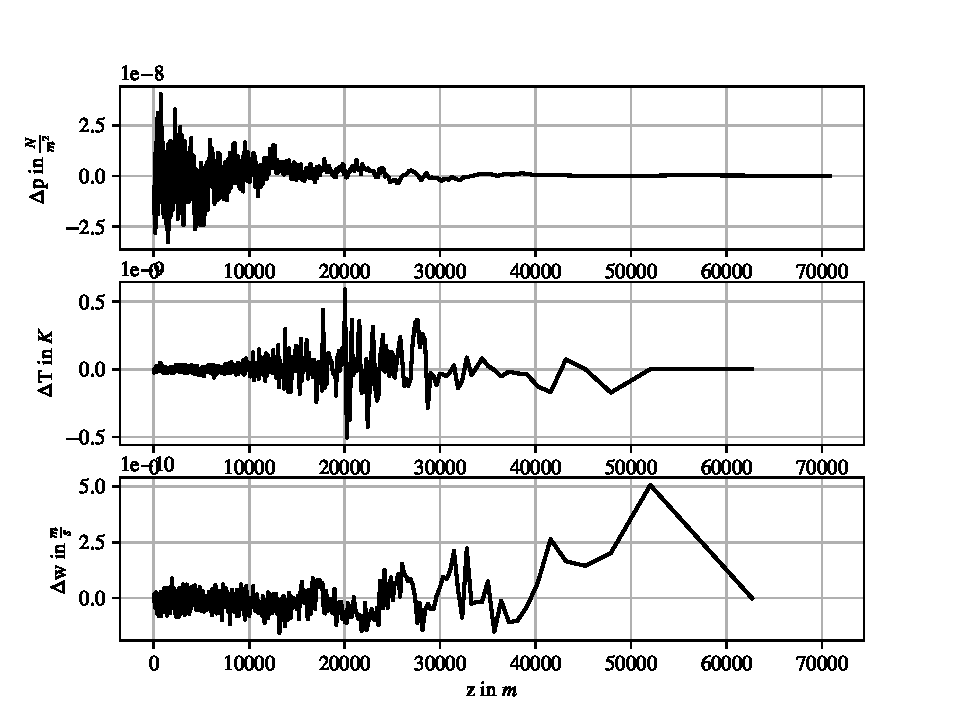
\includegraphics[width=1.2\textwidth]{figures/cp_240s_stat.pdf}}
    \caption{Error (deviation from stationary solution) made using RK4, time-step-size $2.5ms$, and $1000$ grid points, after $240s$ of simulation time on Charney-Phillips grid}
    \label{fig:cp_stat_err}
\end{figure}